\chapter{Introduction to Ladder Logic}
\section{Background of Ladder Logic}
\label{section:ladderlogic}

\begin{figure}[htp]
    \centering
    \includegraphics[width=\imgsmlphoto]{./images/lltoggle_light.png}
    \caption{Togglable Light in Ladder Logic}
    \label{fig:lltoggle_light}
\end{figure}

%docment link: http://www.plcs.net/chapters/whatis1.htm
%reasons for development
Ladder logic was originally developed to replace physical relays used in PLC's.
As a result the ``language'' resembles a circuit diagram. The left most
and right most ``rung'' represent power rails analogous to GND\glossary{name={GND}, description={Ground (or negative in electronics)}} (or negative)
 and VCC\glossary{name={VCC}, description={Voltage at the Common Collector (or postitive voltage in electronics)}} (or positive) what's
placed in between those rungs are the load components \cite{ebookmorris}. In 
the case of programming, the entire logic is created from loads you place 
in between these power rails. Each horizontal ``rung'' is then its own
independent electrical circuit.

Several conventions exist, for example power always flows from left 
to right along each rung. Power also flows from top to bottom along the 
rails. This is counter intuitive since Ladder Logic is suppose to be 
analogous to a circuit schematic and a circuit is simply energized
with no implicit power flow direction. In addition each run must 
start with inputs and end
with exactly one output. Any device that is on a rung is shown in its
initial state. This can be open or closed for inputs.

Modern PLC's operate more like a traditional micro controller and thus the 
original schematic based language can prove to be awkward to work with.

The inputs in Ladder Logic are referred to as loads. A normally open input
is represented by the 
symbol $-\vert ~ ~ \vert-$, and a normally closed input by $-\vert/\vert-$.
In addition an address is usually assigned to each input referring to 
which port on the physical PLC the input is connected to. Logical AND 
can be formed by having two logical loads on one rung \cite{ebookmorris}. 
Similarly logical OR can be formed by creating a branch along one 
rung as shown in Figure \ref{fig:intro_fig3a}.

We can define the language of Ladder Logic as follows $Q = \langle M,S,C,R,P \rangle $

\begin{itemize}
	\item M: set of monitored variables.
	\item S: set of state variables.
	\item C: set of controlled outputs.
	\item R: set of rungs.
	\item P: set of power rails.
\end{itemize}

\begin{figure}[htp]
    \centering
    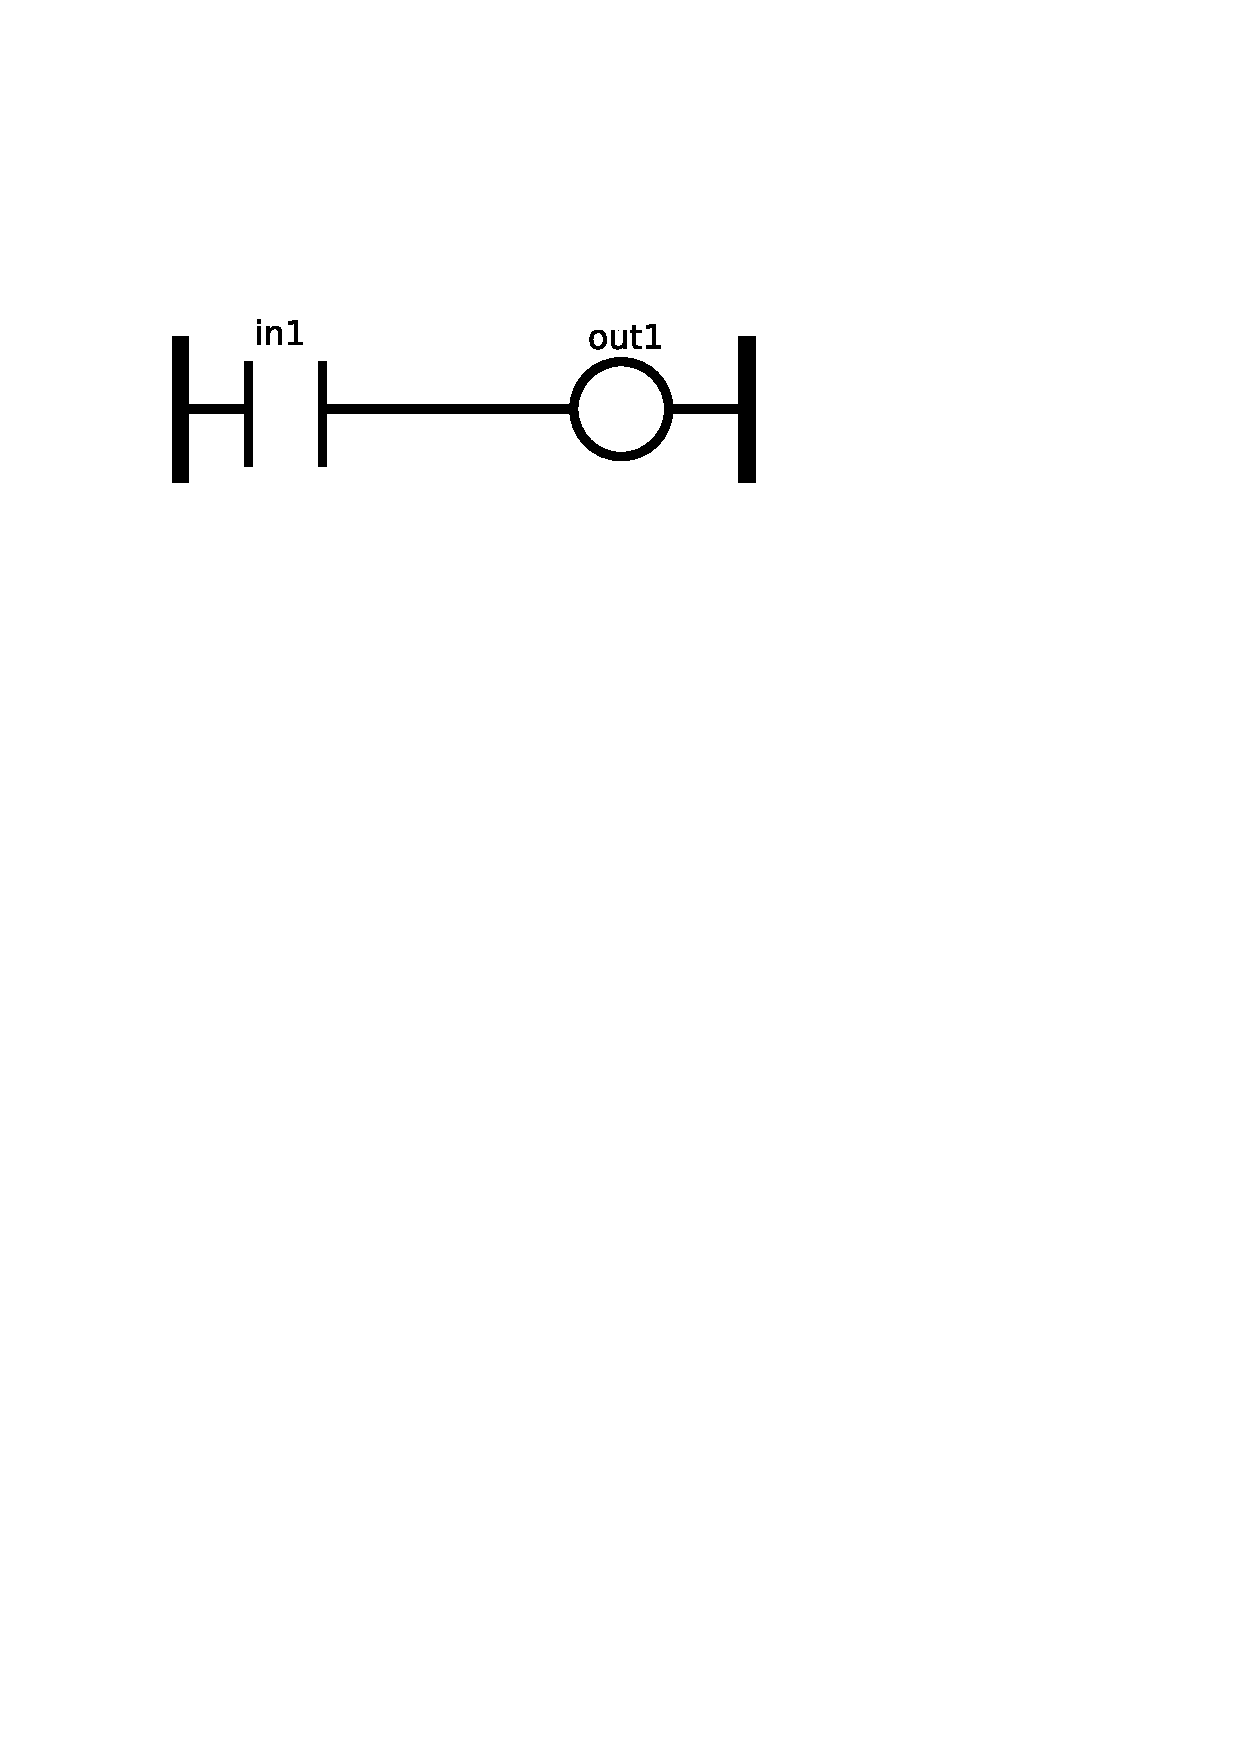
\includegraphics[width=\imgsmall]{./images/intro_fig1.png}
    \caption{Basic Ladder Logic Diagram}
    \label{fig:intro_fig1}
\end{figure}

The most basic structure of Ladder Logic is shown in Figure \ref{fig:intro_fig1}. 
We have 
$$M=\lbrace in_1 \rbrace, S=\lbrace out_1 \rbrace, C=\lbrace out_1 \rbrace, R=\lbrace rung_1 \rbrace, P=\lbrace L,R \rbrace.$$
Note that $rung_1$ is not explicitly labelled in Ladder Logic but we give it a name here
so we may refer to it and complete our model.

\clearpage
The semantics of Figure \ref{fig:intro_fig1} is then given by: 
\begin{table}[h]
    \centering
    \begin{tabular}{|l|l|l|}
        \hline
        Action & Result \\
        \hline
        $@T(in_1 = true)$ & $out_1 := true$ \\
        \hline
        $@T(in_1 = false)$ & $out_1 := false$ \\
        \hline
    \end{tabular}
    \caption{Semantics for Fig \ref{fig:intro_fig1}}
    \label{table:table_for_fig1}
\end{table}


Where $@T(<condition>)$ is used to denote the positive edge of a condition becoming true.
We also assume negligible delay between the action occurring and the result being asserted.
It is important to note that our function table must be complete that is have an entry for
all possible combinations in the input domain.

\begin{figure}[h]
    \centering
    \includegraphics[width=\imgsmall]{./images/intro_fig2.png}
    \caption{Simple AND Logic Diagram}
    \label{fig:intro_fig2}
\end{figure}

When multiple inputs are connected on the same rung it is interpreted as a logical AND 
expression. In Figure \ref{fig:intro_fig2} we can expand our model to:

$$M=\lbrace in_1, in_2 \rbrace, S=\lbrace out_1 \rbrace, C=\lbrace out_1 \rbrace, R=\lbrace rung_1 \rbrace, P=\lbrace L,R \rbrace.$$

We can see that both $in_1$ and $in_2$ are on $rung_1$. This is interpreted as follows:

\begin{table}[h]
    \centering
       \begin{tabular}{|l|l|l|}
        \hline
        Action & Result \\
        \hline
        $Initial$ & $in_1 := false, in_2 := false, out_1 := false$\\
        \hline
        $@T(in_1 = true \wedge in_2 = true)$ & $out_1 := true$ \\
        \hline
        $@T(in_1 = false \vee in_2 = false)$ & $out_1 := false$ \\
        \hline
    \end{tabular}
    \caption{Semantics for Fig \ref{fig:intro_fig2}}
    \label{table:table_for_fig2}
\end{table}

The conditions $in_1$ and $in_2$ are combined to form our composed action $@T(in_1 = true \wedge in_2 = true)$ 
as seen in Table \ref{table:table_for_fig2}. We also note that there is no action for each individual condition
becoming true nor do we need to individually calculate the timing on $in_1$ or $in_2$.

\begin{figure}[h]
    \centering
    \includegraphics[width=\imgsmall]{./images/intro_fig3.png}
    \caption{Branching Rungs}
    \label{fig:intro_fig3}
\end{figure}


In addition to multiple inputs connected to the same rung, inputs can also be branched. A branched rung as
show in Figure \ref{fig:intro_fig3} behaves like a logical OR. In addition two or more rungs can be joined
as shown in Figure \ref{fig:intro_fig3a}. The semantics are equivalent for both Figure \ref{fig:intro_fig3} and Figure \ref{fig:intro_fig3a}.

\begin{figure}[h]
    \centering
    \includegraphics[width=\imgsmall]{./images/intro_fig3a.png}
    \caption{Branching Rungs (Alternative)}
    \label{fig:intro_fig3a}
\end{figure}

\begin{table}[h]
    \centering
       \begin{tabular}{|l|l|l|}
        \hline
        Action & Result \\
        \hline
        $Initial$ & $in_1 := false, in_2 := false, out_1 := false$\\
        \hline
        $@T_n(in_1 = true \vee in_2 = true)$ & $out_1 := true$ \\
        \hline
        $@T_n(in_1 = false \wedge in_2 = false)$ & $out_1 := false$\\
        \hline
    \end{tabular}
    \caption{Semantics for Fig \ref{fig:intro_fig3} and Fig \ref{fig:intro_fig3a}}
    \label{table:table_for_fig3}
\end{table}

Since the semantics are the same for both Figure \ref{fig:intro_fig3} and Figure \ref{fig:intro_fig3a} we can
express both outcomes with function Table \ref{table:table_for_fig3}.
As before in Table \ref{table:table_for_fig2} in Table \ref{table:table_for_fig3} $in_1$ and $in_2$ are composed to form our composed action $@T(in_1 = true \vee in_2 = true)$. However it is also possible to represent this in another way as we will show below.

\begin{table}[h]
    \centering
       \begin{tabular}{|l|l|l|}
        \hline
        Action & Result \\
        \hline
        $Initial$ &$in_1 := false, in_2 := false, out_1 := false$\\
        \hline
        $@T(in_1 = true)$ & $out_1 := true$ \\
        \hline
        $@T(in_2 = true)$ & $out_1 := true$ \\
        \hline
        $@T(in_1 = false \wedge in_2 = false)$ & $out_1 := false$\\
        \hline
    \end{tabular}
    \caption{Semantics for Fig \ref{fig:intro_fig3} and Fig \ref{fig:intro_fig3a}}
    \label{table:table_for_fig3a}
\end{table}

In Table \ref{table:table_for_fig3a} we choose to represent $in_1$ and $in_2$ as separate inputs. This matches Figure
\ref{fig:intro_fig3a} more closely but also makes any verification harder than Table \ref{table:table_for_fig3}. For
smaller examples Table \ref{table:table_for_fig3} make more sense since you can verify relatively simple smaller functions
quite fast. If a system becomes reasonably large however there might be motivation to use the style shown in 
Table \ref{table:table_for_fig3a} since it will allow more complex functions to be decomposed into simpler inputs.
Since semantically the two are equivalent this thesis will focus to the first convention.


\begin{figure}[h]
    \centering
    \includegraphics[trim= 0 140mm 40mm 10mm, clip, width=250px]{./images/intro_and_graph.pdf} %custom size
    \caption{State diagram conversion for Table \ref{table:table_for_fig2}}
    \label{fig:intro_and_graph}
\end{figure}

A rung can be defined as a directed graph with exactly one $rung_1(start)$ and one $rung_1(end)$. The state variables form guard conditions along the edges. A branch in this case represents 2 edges leaving one node. For example Figure \ref{fig:intro_fig2}
can be easily converted into a state diagram by observing the results in Table \ref{table:table_for_fig2}. 
Each row of Table \ref{table:table_for_fig2} is directly converted into an edge with the appropriate guard conditions.
Each output assertion is given their own state. Finally in Figure \ref{fig:intro_and_graph} we observe the start state of the rung, and the end state for the rung. In Ladder Logic each rung is executed continuously with each scan, therefore it is necessary to also add an loop from $rung_1(end)$ to $rung_1(start)$. We can similarily take Figure \ref{fig:intro_fig3} observe its Function Table \ref{table:table_for_fig3} and produce a state diagram from its function table. Figure \ref{fig:intro_or_graph} represents said construction.


\begin{figure}[h]
    \centering
    \includegraphics[trim= 00mm 140mm 40mm 10mm, clip, width=250px]{./images/intro_or_graph.pdf} %custom size
    \caption{State diagram conversion for Table \ref{table:table_for_fig3}}
    \label{fig:intro_or_graph}
\end{figure}

Thus, each rung can be converted into an equivalent state diagram by examining its 
function table, assigning the state variables to guard conditions, and creating a
state for each of the outputs. For thoroughness we complete this procedure to produce
a state diagram shown in Figure \ref{fig:intro_or_graph_3a} which is a representation of 
Figure \ref{fig:intro_fig3a} and its
corresponding Table \ref{table:table_for_fig3a}.


\begin{figure}[h]
    \centering
    \includegraphics[width=\imgmedsmall]{./images/intro_or_graph_3a.pdf} %custom size
    \caption{State diagram conversion for Table \ref{table:table_for_fig3a}}
    \label{fig:intro_or_graph_3a}
\end{figure}

Another concept in ladder logic is latching. Suppose you have a light that you want to be able to turn on and stay on after you push a button. With any of the ladder diagrams shown above the light would go out as soon as the buttons were all released. In order to keep the light on and constantly on after the button is pressed we introduce the latch. We modify our diagram shown in Figure \ref{fig:intro_fig3a} making the output feed back into one of the inputs to our OR circuit. The result is show in Figure~\ref{fig:intro_fig_latched}.

%figure for latched circuits 
\begin{figure}[h]
    \centering
    \includegraphics[width=\imgsmall]{./images/intro_fig_latched.png} 
    \caption{Latched Ladder Logic circuit.}
    \label{fig:intro_fig_latched}
\end{figure}

The latched circuit operates the same way as the behaviour show in Table \ref{table:table_for_fig3a}; the key difference is the feedback of the OR circuit replaces the second row of the function table. This causes $latched\_out1$ to stay on after the initial input is removed.

All Ladder Logic programs are built of these basic primitives in addition each manufacturer offers their own convenience functions and additional blocks. These allow operations like add, subtract, and taking a measurement to be done in one block rather than attempt to construct it through the circuit diagram.
